{\color{indiagreen}\subsection{Trenje in lepenje}}
Telo miruje na vodoravni podlagi.\\
\begin{center}
	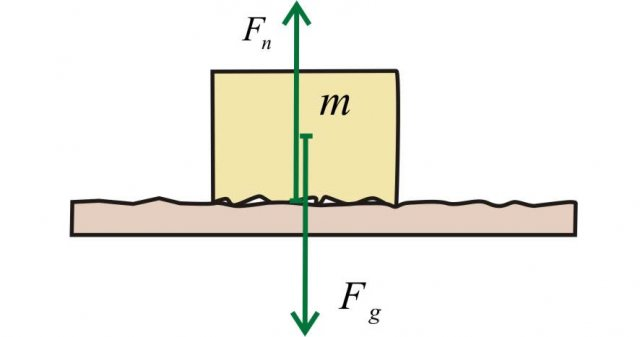
\includegraphics[width=8cm, height=5cm,keepaspectratio=true]{telo_miruje.jpg}
\end{center}
\textbf{$F_g$} - teža je volumsko porazdeljena sila, narišemo jo z prijemališčem v sredini.\\
\textbf{$F_n$} - sila podlage je ploskovno razdeljena in jo narišemo s prejemališčem na sredini ploskve.\\
Telo še zmeraj miruje.
\begin{center}
	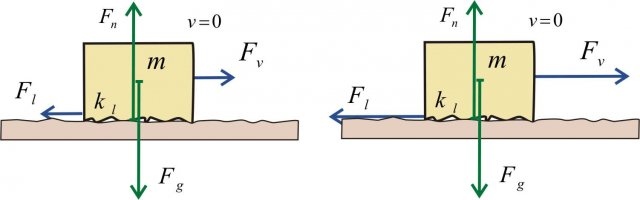
\includegraphics[width=16cm, height=9cm,keepaspectratio=true]{trenje_in_lepenje.jpg}
\end{center}
Sila podlage je sestavljena iz vzdolžne komponente in sile normale. \\
Če povečujemo vlečno silo se spreminja samo vzdolžna komponenta sile podlage.
\begin{align*}
	0 <= F' < F_l\\
\end{align*}
\textbf{$F_l$}- sila lepenja\\
\begin{align*}
	F_l &= k_lN\\
\end{align*}
\textbf{$k_l$} - koeficijent lepenja, je neko število brez enote, ki je odvisen samo od hrapavosti stičnih ploskev podlage in telesa\\
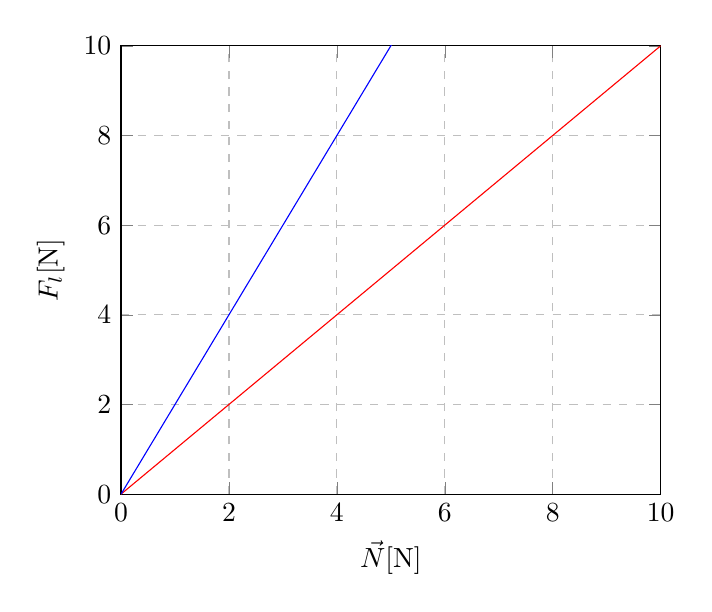
\begin{tikzpicture}
	\begin{axis}[
	    xlabel={$\vec{N}$[N]},
	    ylabel={$F_l$[N]},
	    xmin=0, xmax=10,
	    ymin=0, ymax=10,
	    xtick={0,2,4,6,8,10},
	    ytick={0,2,4,6,8,10},
	    yticklabels={0,2,4,6,8,10},
	    ymajorgrids=true,
	    xmajorgrids=true,
	    grid style=dashed,
	]
	 
	\addplot[domain=0:10,red] {x};
	\addplot[domain=0:10,blue] {2*x};

	\end{axis}
\end{tikzpicture}

Telo se giblje:\\
\textbf{$F_{tr}$} - sila trenja
\begin{align*}
	F_{tr} &= k_{tr}N\\
\end{align*}
\textbf{$k_{tr}$} - koeficijent trenja
\begin{align*}
	k_{tr} < k_l\\
\end{align*}
Je vedno manjši, ker zato da \textbf{premaknemo telo} potrebujemo več sile, ker moramo pretrgati \textbf{medmulekulske vezi} in potem, ko se telo enkrat premika teh vezi ni več in je manjši koeficijent.\\